% Commenti speciali

% !TEX encoding = UTF-8 Unicode
% !TEX TS-program = pdflatex
% !TEX spellcheck = it-IT
% !TEX root = Dispensa/afed.tex

% Capitolo 4
\chapter{Teoremi di punto fisso}\label{Teoremi di punto fisso}
\section{Introduzione}
Possedere condizioni sufficienti riguardo l'esistenza di punti fissi è fondamentale per un analista; in particolare, comunque, sarà indispensabile nell'ambito dell'Analisi non lineare, come vedremo nel capitolo \ref{Alcuni elementi di Analisi non lineare}. Un primo risultato, già noto dal corso di Analisi Matematica II, è il Teorema delle contrazioni.

\begin{teorema}\emph{\textbf{(di Banach--Caccioppoli)}}\index[analitico]{teorema!delle contrazioni}\index[analitico]{teorema!di Banach--Caccioppoli}
	Siano $(X,d)$ uno spazio metrico completo non vuoto ed $f: X \to X$ un'applicazione lipschitziana di costante $C \in \left[ 0,1\right[ $. Allora esiste uno ed un solo $\xi \in X$ tale che $f(\xi) = \xi$.
\end{teorema}
\begin{proof}
	Omettiamo la dimostrazione.
\end{proof}
Miriamo, nel corso di questo capitolo a studiare nel dettaglio altri risultati di questo tipo, sia in dimensione finita che infinita, e ad analizzare alcune prime notevoli applicazioni.
\section{Risultati in dimensione finita}
Il Teorema seguente è stato pubblicato per la prima volta nel $1912$ su \emph{Mathematische Annalen} da Luitzen Egbertus Jan "Bertus" Brouwer. Qui riportiamo una dimostrazione semplificata rispetto all'originale dovuta a John Milnor e, successivamente, rivista da Claude Ambrose Rogers.
\begin{teorema}\emph{\textbf{(di Brouwer)}}\index[analitico]{teorema!di Brouwer}
	Siano $K \subseteq \R^n$ convesso, compatto e non vuoto ed $f: K \to K$ un'applicazione continua. Esiste $x \in K$ tale che $f(x) = x$.
\end{teorema}
\begin{proof}
	Vediamo innanzitutto il caso $K = \overline{\B(0,1)}$. Mostriamo che non esiste alcuna applicazione $f: \overline{\B(0,1)} \to \partial \B(0,1)$ di classe $C^1$ tale che per ogni $x \in \partial \B(0,1)$ si abbia $f(x) = x$. Supponiamo, per assurdo, che una tale applicazione esista. Per ogni $x \in \overline{\B(0,1)}$ e per ogni $t \in [0,1]$ sia $f_t(x) = (1-t)x + tf(x)$. Osserviamo che
	\[ \abs{f_t(x)} \le (1-t)\abs{x} +t\abs{f(x)} \le (1-t) +t = 1, \]
	perciò $\textup{Im}(f_t)\subseteq \overline{\B(0,1)}$. Inoltre, se $x \in \partial \B(0,1)$,
	\[ f_t(x) = (1-t)x + tx = x. \]
	Detta $g(x) = f(x) - x$, si ha $f_t(x) = x + tg(x)$. Essendo $f$ di classe $C^1$ su $\overline{\B(0,1)}$,  tale è pure $g$, quindi, per la disuguaglianza di Lagrange ed il Teorema di Weierstrass, per ogni $x_1,x_2 \in \overline{\B(0,1)}$
	\[ \abs{g(x_2) - g(x_1)} \le \norm{dg}_\infty \abs{x_2 - x_1} \le C \abs{x_2 - x_1}, \]
	quindi $g$ è lipschitziana su $\overline{\B(0,1)}$. Se ora $x_1,x_2 \in \overline{\B(0,1)}$ tali che $f_t(x_1) = f_t(x_2)$, allora 
	\[ x_2 - x_1 = t(g(x_1 - g(x_2))), \]
	quindi 
	\[ \abs{x_2 - x_1} = t\abs{g(x_1) - g(x_2)} \le Ct \abs{x_2 - x_1}. \]
	In particolare, se $t \in \left[ 0,\frac{1}{C}\right[$, l'unica possibilità è che $x_1 = x_2$, altrimenti otterrei $t \ge \frac{1}{C}$, che sarebbe assurdo. In altre parole, per $t \in \left[ 0,\frac{1}{C}\right[$ $f_t$ è iniettiva. Osserviamo anche che per ogni $x \in \B(0,1)$
	\[ df_t(x) = \textup{Id} + tdg(x) \]
	quindi, essendo $g$ di classe $C^1$, esiste $t_0 \in  \left[ 0,\frac{1}{C}\right[$ tale che per ogni $t \in \left[ 0,t_0\right] $ e per ogni $x \in \B(0,1)$ si abbia $\det(df_t(x)) > 0$ che, in altre parole, significa che $df_t(x)$ è biettivo.\footnote{In generale, siano $A,B \in \textup{Mat}_n(\R)$ tali che $\det(A) > 0$ ed $a \in \R$. Consideriamo $\varphi: \left[ 0, a\right[ \to \R$ tale che $\varphi(t) = \det(A + tB)$. Essendo $\det$ un'applicazione continua, per composizione anche $\varphi$ è una funzione continua. In particolare è continua in $0$. Dal fatto che $\varphi(0) = \det(A) > 0$, per il Teorema della permanenza del segno, esiste $t_0 \in  \left[ 0,a\right[$ tale che per ogni $t \in \left[ 0,t_0\right]$ si abbia $\varphi(t) > 0$.} Per il Teorema di inversione locale, per ogni $t \in \left[ 0,t_0\right]$ e per ogni $x \in \B(0,1)$ esiste un intorno aperto $U_x$ di $x$ in $\B(0,1)$ tale che $f_t(U_x)$ sia aperto. In particolare, per ogni $t \in \left[ 0,t_0\right] $, siccome
	\[ G_t = f_t(\B(0,1)) = \bigcup_{x \in \B(0,1)} f_t(U_x),\]
	possiamo affermare che $G_t$ è aperto. Osserviamo che, in realtà, per ogni $t \in \left[ 0,t_0\right] $ si ha $G_t = \B(0,1)$. Infatti, se per assurdo così non fosse, allora esisterebbe $y_0 \in \partial G_t \cap \B(0,1)$. Sia allora $(x_h)$ in $\B(0,1)$ tale che $f_t(x_h) \to y_0$. Per compattezza, esiste $x_0 \in \overline{\B(0,1)}$ tale che, a meno di sottosuccessioni, $x_h \to x_0$. Allora, per continuità di $f_t$ ed unicità del limite, $f_t(x_0) = y_0$. Dal fatto che $G_t$ è aperto dovrebbe essere allora $x_0 \in \partial \B(0,1)$, ma quindi $y_ 0 = f_t(x_0) = x_0 \in \partial \B(0,1)$, che da la contraddizione. Possiamo quindi affermare che $f_t: \overline{\B(0,1)} \to \overline{\B(0,1)}$ è biettiva per ogni $t \in [0,t_0]$. Detta $F: [0,1] \to \R$ tale che
	\[ F(t) = \int_{B(0,1)} \det(df_t(x)) d\mathcal{L}^n(x), \]
	per la formula dell'area, per $t \in [0,t_0]$ si ha 
	\[ F(t) = \int_{B(0,1)} \abs{\det(df_t)} d\mathcal{L}^n = \int_{f_t(\B(0,1))} d\mathcal{L}^n = \mathcal{L}^n(f_t(\B(0,1))) = \mathcal{L}^n(\B(0,1)),  \]
	ossia $F$ è costante su $[0,t_0]$. Essendo, per definizione di determinante, $F$ un polinomio in $t$, allora è costante, quindi per ogni $t \in [0,1]$
	\[ F(t) = \mathcal{L}^n(\B(0,1)). \]
	In particolare, $F(1)> 0$. Ma, per ogni $x \in \overline{\B(0,1)}$ si ha $f_1(x) = f(x) \in \partial \B(0,1)$, quindi 
	\[ (f_1(x) | f_1(x)) = \abs{f_1(x)}^2=1. \]
	Preso $v \in \R^n$ tale che $x+tv \in \overline{\B(0,1)}$, 
	\[ 2(df_1(x)v | f_1(x)) = \frac{d}{dt} (f_1(x+tv) | f_1(x+tv))|_{t=0} = \frac{d}{dt} 1|_{t=0} = 0. \]
	Allora, $\textup{Im}(df_1(x)) \subseteq \textup{span}(f(x))^\perp$. Siccome $\dim (\textup{span}(f(x))) = 1$, allora per ogni $x \in \B(0,1)$ si ha $\textup{rg}(df_1(x)) \le n-1$. In particolare, per ogni $x \in \B(0,1)$ deve essere $\det(df_1(x)) = 0$. Allora $F(1) = 0$, assurdo.
	
	Ora, per il Teorema di Stone--Weierstrass, esiste una successione $(p_h)$ di applicazioni a componenti polinomiali tale che $p_h \to f$ uniformemente su $\overline{\B(0,1)}$. In particolare, esiste $M>0$ tale che per ogni $h \in \N$
	\[ \abs{p_h(x)} \le \abs{p_h(x) - f(x)} + \abs{f(x)} \le M, \]
	quindi $\norm{p_h} \le M$. Posto $\psi_h(x) = M^{-1} p_h(x)$ si ha $\norm{\psi_h}_\infty \le 1$, ossia $\textup{Im}(\psi_h) \subseteq \overline{\B(0,1)}$. Per assurdo, supponiamo che $\psi_h(x) \ne x$ per ogni $x \in \overline{\B(0,1)}$. Definiamo $f_h: \overline{\B(0,1)} \to \partial \B(0,1)$ di classe $C^1$ tale che $f_h(x)$ sia l'intersezione della semiretta uscente da $\psi_h(x)$, e passante per $x$, con $\partial \B(0,1)$.\footnote{Il fatto che sia di classe $C^1$ viene dal fatto che $\psi_h$ è di classe $C^1$ e la costruzione geometrica non provoca perdita di regolarità.}
	
	\begin{center}
		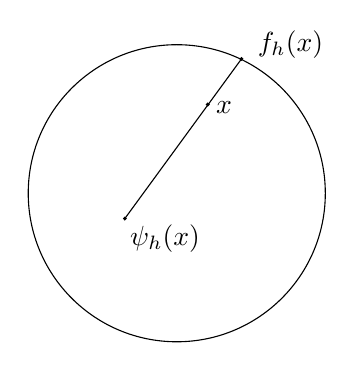
\begin{tikzpicture}[x=0.5pt,y=0.5pt,yscale=-1,xscale=1]
			%uncomment if require: \path (0,316); %set diagram left start at 0, and has height of 316
			
			%Shape: Circle [id:dp5526126125166915] 
			\draw   (203.5,154.25) .. controls (203.5,94.96) and (251.56,46.9) .. (310.85,46.9) .. controls (370.14,46.9) and (418.2,94.96) .. (418.2,154.25) .. controls (418.2,213.54) and (370.14,261.6) .. (310.85,261.6) .. controls (251.56,261.6) and (203.5,213.54) .. (203.5,154.25) -- cycle ;
			%Shape: Circle [id:dp3136828089910624] 
			\draw  [fill={rgb, 255:red, 0; green, 0; blue, 0 }  ,fill opacity=1 ] (272.4,172.53) .. controls (272.4,172.02) and (272.82,171.6) .. (273.33,171.6) .. controls (273.85,171.6) and (274.27,172.02) .. (274.27,172.53) .. controls (274.27,173.05) and (273.85,173.47) .. (273.33,173.47) .. controls (272.82,173.47) and (272.4,173.05) .. (272.4,172.53) -- cycle ;
			%Shape: Circle [id:dp8432142275934196] 
			\draw  [fill={rgb, 255:red, 0; green, 0; blue, 0 }  ,fill opacity=1 ] (332.27,90.13) .. controls (332.27,89.62) and (332.68,89.2) .. (333.2,89.2) .. controls (333.72,89.2) and (334.13,89.62) .. (334.13,90.13) .. controls (334.13,90.65) and (333.72,91.07) .. (333.2,91.07) .. controls (332.68,91.07) and (332.27,90.65) .. (332.27,90.13) -- cycle ;
			%Straight Lines [id:da2597269370190327] 
			\draw    (357.6,57.2) -- (273.33,172.53) ;
			%Shape: Circle [id:dp9542475070772747] 
			\draw  [fill={rgb, 255:red, 0; green, 0; blue, 0 }  ,fill opacity=1 ] (356.67,57.2) .. controls (356.67,56.68) and (357.08,56.27) .. (357.6,56.27) .. controls (358.12,56.27) and (358.53,56.68) .. (358.53,57.2) .. controls (358.53,57.72) and (358.12,58.13) .. (357.6,58.13) .. controls (357.08,58.13) and (356.67,57.72) .. (356.67,57.2) -- cycle ;
			
			% Text Node
			\draw (275.33,175) node [anchor=north west][inner sep=0.75pt]  {$\psi _{h}( x)$};
			% Text Node
			\draw (337.33,86.4) node [anchor=north west][inner sep=0.75pt]  {$x$};
			% Text Node
			\draw (367.6,35) node [anchor=north west][inner sep=0.75pt]  {$f_{h}( x)$};
			
			
		\end{tikzpicture}
	\end{center}
	Se $x \in \partial \B(0,1)$ risulta $f_h(x)= x$, assurdo.\footnote{La costruzione geometrica effettuata qui gioca un ruolo fondamentale: se avessimo preso l'altra intersezione che la retta passante per $\psi_h(x)$ e $x$ ha con $\partial \B(0,1)$, non avremmo questa proprietà. Inoltre questo modo di arrivare ad un assurdo giustifica l'utilizzo del Teorema di Stone--Weierstrass in quanto necessitiamo di funzioni di classe $C^1$.} Quindi, per ogni $h \in \N$ esiste $x_h \in \overline{\B(0,1)}$ tale che $\psi_h(x_h) = x_h$. Dal fatto che $\overline{\B(0,1)}$ è compatto, a meno di sottosuccessioni, $x_h \to x \in \overline{\B(0,1)}$. Ora, siccome $p_h \to f$ uniformemente, anche $\psi_h \to f$ uniformemente. In particolare, da 
	\[ \abs{\psi_h(x_h) - f(x)} \le \abs{\psi_h(x_h) - f(x_h)} + \abs{f(x_h)-f(x)} \le \norm{\psi_h -f}_\infty + \abs{f(x_h)-f(x)}\]
	e dalla continuità di $f$, 
	\[ \lim\limits_{h} \psi_h(x_h) = f(x), \]
	ma 
	\[ \lim\limits_{h} \psi_h(x_h) = \lim\limits_{h} x_h = x \]
	da cui $f(x) = x$.
	
	Quanto appena dimostrato si generalizza immediatamente al caso $K= \overline{\B(0,R)}$ per $R > 0$. Nel caso generale, sia $R > 0$ tale che $K \subseteq \overline{B(0,R)}$. Essendo $\R^n$ uno spazio di Hilbert e $K$ convesso, chiuso, in quanto compatto, e non vuoto, l'applicazione $P_K: \R^n \to K$, tale che per ogni $x \in \R^n$ $P_K(x)$ è la proiezione ortogonale di $x$ su $K$, è lipschitziana di costante $1$. In particolare è continua. Se consideriamo l'applicazione $f \circ P_K : \overline{\B(0,R)} \to \overline{\B(0,R)}$, anch'essa continua per composizione, per quanto visto precedentemente, esiste $x \in \overline{\B(0,R)}$ tale che $f(P_k(x)) = x$. Allora $x \in \textup{Im}(f)$, ossia $x \in K$, quindi $P_K(x) = x$ che conduce a $f(x) = x$, che è la tesi.
\end{proof}

\begin{osservazione}
	Siano $a<b$ ed $f: [a,b] \to [a,b]$ un'applicazione continua. In questa situazione la dimostrazione può essere molto semplificata, riconducendo il Teorema di Brouwer al Teorema di esistenza degli zeri. Se consideriamo infatti la funzione ausiliaria $\varphi: [a,b] \to [a,b]$ tale che 
	\[ \varphi(x) = f(x) - x. \]
	Chiaramente $\varphi$ è continua e, siccome $\textup{Im}(f) \subseteq [a,b]$, 
	\begin{align*}
		\varphi(b) &= f(b) - b \le 0 & &\textup{e} &  \varphi(a) &= f(a) - a \ge 0.
	\end{align*} 
	Se $\varphi(a) = 0$ (risp. $\varphi(b) = 0$), allora $f(a) = a$ (risp. $f(b) = b$). Se invece $\varphi(a),\varphi(b) \ne 0$, allora $\varphi(a) \varphi(b) < 0$ e, per il Teorema di esistenza degli zeri, esiste $x \in \left] a,b\right[ $ tale che $\varphi(x) = 0$, ossia $f(x) = x$.
\end{osservazione}

\begin{corollario}
	Sia $\overline{\B(0,1)} \subseteq \R^n$. Non esiste alcuna applicazione $f: \overline{\B(0,1)} \to \partial \B(0,1)$ continua tale che per ogni $x \in \partial \B(0,1)$ si abbia $f(x) = x$.
\end{corollario}
\begin{proof}
	Supponiamo, per assurdo, che tale applicazione $f: \overline{\B(0,1)} \to \partial \B(0,1)$ esista. Sia allora $g: \overline{\B(0,1)} \to \overline{\B(0,1)}$ tale che
	\[ g(x) = -f(x). \]
	Per il Teorema di Brouwer, esiste $x \in \overline{\B(0,1)}$ tale che $g(x) = x$. Essendo $\partial \B(0,1)$ simmetrico rispetto a $0$, risulta $\textup{Im}(g) \subseteq \partial \B(0,1)$ allora $x \in \partial \B(0,1)$ e \[ x = g(x) = -f(x) = -x, \] 
	da cui l'assurdo.
\end{proof}

Analizziamo alcune importanti applicazioni del Teorema di Brouwer. La prima è il Teorema di invarianza del dominio, per cui è necessaria una premessa di carattere topologico.
\begin{definizione}
	Consideriamo $(X,\tau)$ uno spazio topologico. Distinguiamo le seguenti proprietà di separazione:
	\begin{itemize}
		\item diciamo che $(X,\tau)$ è $T_0$\index[analitico]{spazio!topologico!$T_0$}\index[simboli]{$T_0$} se per ogni $x,y \in X$ tali che $x\ne y$, esiste $U \in \tau$ tale che $x \in U$ e $y\notin U$,
		\begin{center}
			\begin{tikzpicture}[x=0.75pt,y=0.75pt,yscale=-1,xscale=1]
				%uncomment if require: \path (0,300); %set diagram left start at 0, and has height of 300
				
				%Shape: Circle [id:dp1732517118606005] 
				\draw  [fill={rgb, 255:red, 0; green, 0; blue, 0 }  ,fill opacity=1 ] (205,150) .. controls (205,149.45) and (205.45,149) .. (206,149) .. controls (206.55,149) and (207,149.45) .. (207,150) .. controls (207,150.55) and (206.55,151) .. (206,151) .. controls (205.45,151) and (205,150.55) .. (205,150) -- cycle ;
				%Shape: Polygon Curved [id:ds020722407137701016] 
				\draw  [dash pattern={on 0.84pt off 2.51pt}] (160,119) .. controls (149,85.6) and (206,95.4) .. (250,119) .. controls (294,142.6) and (230,149) .. (250,179) .. controls (270,209) and (185,218.6) .. (165,188.6) .. controls (145,158.6) and (171,152.4) .. (160,119) -- cycle ;
				%Shape: Circle [id:dp19705533391128083] 
				\draw  [fill={rgb, 255:red, 0; green, 0; blue, 0 }  ,fill opacity=1 ] (315,156) .. controls (315,155.45) and (315.45,155) .. (316,155) .. controls (316.55,155) and (317,155.45) .. (317,156) .. controls (317,156.55) and (316.55,157) .. (316,157) .. controls (315.45,157) and (315,156.55) .. (315,156) -- cycle ;
				
				% Text Node
				\draw (191,132.4) node [anchor=north west][inner sep=0.75pt]    {$x$};
				% Text Node
				\draw (220,84.4) node [anchor=north west][inner sep=0.75pt]    {$U$};
				% Text Node
				\draw (301,138.4) node [anchor=north west][inner sep=0.75pt]    {$y$};
				
				
			\end{tikzpicture}
		\end{center}
		\item diciamo che $(X,\tau)$ è $T_1$\index[analitico]{spazio!topologico!$T_1$}\index[simboli]{$T_1$} se per ogni $x,y \in X$ tali che $x\ne y$, esistono $U,V \in \tau$ tali che $x \in U$, $y \notin U$, $x \notin V$ e $y \in V$,
		\begin{center}
			\begin{tikzpicture}[x=0.75pt,y=0.75pt,yscale=-1,xscale=1]
				%uncomment if require: \path (0,300); %set diagram left start at 0, and has height of 300
				
				%Shape: Circle [id:dp1732517118606005] 
				\draw  [fill={rgb, 255:red, 0; green, 0; blue, 0 }  ,fill opacity=1 ] (205,150) .. controls (205,149.45) and (205.45,149) .. (206,149) .. controls (206.55,149) and (207,149.45) .. (207,150) .. controls (207,150.55) and (206.55,151) .. (206,151) .. controls (205.45,151) and (205,150.55) .. (205,150) -- cycle ;
				%Shape: Polygon Curved [id:ds020722407137701016] 
				\draw  [dash pattern={on 0.84pt off 2.51pt}] (160,119) .. controls (149,85.6) and (206,95.4) .. (250,119) .. controls (294,142.6) and (230,149) .. (250,179) .. controls (270,209) and (185,218.6) .. (165,188.6) .. controls (145,158.6) and (171,152.4) .. (160,119) -- cycle ;
				%Shape: Circle [id:dp19705533391128083] 
				\draw  [fill={rgb, 255:red, 0; green, 0; blue, 0 }  ,fill opacity=1 ] (315,156) .. controls (315,155.45) and (315.45,155) .. (316,155) .. controls (316.55,155) and (317,155.45) .. (317,156) .. controls (317,156.55) and (316.55,157) .. (316,157) .. controls (315.45,157) and (315,156.55) .. (315,156) -- cycle ;
				%Shape: Polygon Curved [id:ds3453941623544552] 
				\draw  [dash pattern={on 0.84pt off 2.51pt}] (281,117) .. controls (357,83.2) and (358,79.8) .. (371,117) .. controls (384,154.2) and (413,162.2) .. (371,177) .. controls (329,191.8) and (306,216.6) .. (286,186.6) .. controls (266,156.6) and (205,150.8) .. (281,117) -- cycle ;
				
				% Text Node
				\draw (191,132.4) node [anchor=north west][inner sep=0.75pt]    {$x$};
				% Text Node
				\draw (220,84.4) node [anchor=north west][inner sep=0.75pt]    {$U$};
				% Text Node
				\draw (301,138.4) node [anchor=north west][inner sep=0.75pt]    {$y$};
				% Text Node
				\draw (373,91.4) node [anchor=north west][inner sep=0.75pt]    {$V$};
				
				
			\end{tikzpicture}
		\end{center}
		\item diciamo che $(X,\tau)$ è $T_2$, o \emph{di Hausdorff},\index[analitico]{spazio!topologico!$T_2$}\index[analitico]{spazio!topologico!di Hausdorff}\index[simboli]{$T_2$} se per ogni $x,y \in X$ tali che $x\ne y$, esistono $U,V \in \tau$ tali che $x \in U$, $y \in V$ e $U \cap V = \emptyset$,
		\begin{center}
			\begin{tikzpicture}[x=0.75pt,y=0.75pt,yscale=-1,xscale=1]
				%uncomment if require: \path (0,300); %set diagram left start at 0, and has height of 300
				
				%Shape: Circle [id:dp1732517118606005] 
				\draw  [fill={rgb, 255:red, 0; green, 0; blue, 0 }  ,fill opacity=1 ] (205,150) .. controls (205,149.45) and (205.45,149) .. (206,149) .. controls (206.55,149) and (207,149.45) .. (207,150) .. controls (207,150.55) and (206.55,151) .. (206,151) .. controls (205.45,151) and (205,150.55) .. (205,150) -- cycle ;
				%Shape: Polygon Curved [id:ds020722407137701016] 
				\draw  [dash pattern={on 0.84pt off 2.51pt}] (160,119) .. controls (149,85.6) and (206,95.4) .. (250,119) .. controls (294,142.6) and (230,149) .. (250,179) .. controls (270,209) and (185,218.6) .. (165,188.6) .. controls (145,158.6) and (171,152.4) .. (160,119) -- cycle ;
				%Shape: Circle [id:dp19705533391128083] 
				\draw  [fill={rgb, 255:red, 0; green, 0; blue, 0 }  ,fill opacity=1 ] (315,156) .. controls (315,155.45) and (315.45,155) .. (316,155) .. controls (316.55,155) and (317,155.45) .. (317,156) .. controls (317,156.55) and (316.55,157) .. (316,157) .. controls (315.45,157) and (315,156.55) .. (315,156) -- cycle ;
				%Shape: Polygon Curved [id:ds3453941623544552] 
				\draw  [dash pattern={on 0.84pt off 2.51pt}] (293,130.2) .. controls (319,73.4) and (358,79.8) .. (371,117) .. controls (384,154.2) and (413,162.2) .. (371,177) .. controls (329,191.8) and (265,214.2) .. (286,186.6) .. controls (307,159) and (267,187) .. (293,130.2) -- cycle ;
				
				% Text Node
				\draw (191,132.4) node [anchor=north west][inner sep=0.75pt]    {$x$};
				% Text Node
				\draw (220,84.4) node [anchor=north west][inner sep=0.75pt]    {$U$};
				% Text Node
				\draw (301,138.4) node [anchor=north west][inner sep=0.75pt]    {$y$};
				% Text Node
				\draw (373,91.4) node [anchor=north west][inner sep=0.75pt]    {$V$};
				
				
			\end{tikzpicture}
		\end{center}
		\item diciamo che $(X,\tau)$ è $T_3$, o \emph{regolare},\index[analitico]{spazio!topologico!$T_3$}\index[analitico]{spazio!topologico!regolare}\index[simboli]{$T_3$} se per ogni $x,y \in X$ tali che $x\ne y$, per ogni $C \subseteq X$ chiuso tale che $x \in C$ e $y \notin C$, esistono $U,V \in \tau$ tali che $C \subseteq U$, $y \in V$ e $U \cap V = \emptyset$,
		\begin{center}
			\begin{tikzpicture}[x=0.75pt,y=0.75pt,yscale=-1,xscale=1]
				%uncomment if require: \path (0,300); %set diagram left start at 0, and has height of 300
				
				%Shape: Circle [id:dp1732517118606005] 
				\draw  [fill={rgb, 255:red, 0; green, 0; blue, 0 }  ,fill opacity=1 ] (205,150) .. controls (205,149.45) and (205.45,149) .. (206,149) .. controls (206.55,149) and (207,149.45) .. (207,150) .. controls (207,150.55) and (206.55,151) .. (206,151) .. controls (205.45,151) and (205,150.55) .. (205,150) -- cycle ;
				%Shape: Polygon Curved [id:ds020722407137701016] 
				\draw  [dash pattern={on 0.84pt off 2.51pt}] (160,119) .. controls (149,85.6) and (206,95.4) .. (250,119) .. controls (294,142.6) and (230,149) .. (250,179) .. controls (270,209) and (185,218.6) .. (165,188.6) .. controls (145,158.6) and (171,152.4) .. (160,119) -- cycle ;
				%Shape: Circle [id:dp19705533391128083] 
				\draw  [fill={rgb, 255:red, 0; green, 0; blue, 0 }  ,fill opacity=1 ] (315,156) .. controls (315,155.45) and (315.45,155) .. (316,155) .. controls (316.55,155) and (317,155.45) .. (317,156) .. controls (317,156.55) and (316.55,157) .. (316,157) .. controls (315.45,157) and (315,156.55) .. (315,156) -- cycle ;
				%Shape: Polygon Curved [id:ds3453941623544552] 
				\draw  [dash pattern={on 0.84pt off 2.51pt}] (293,130.2) .. controls (319,73.4) and (358,79.8) .. (371,117) .. controls (384,154.2) and (413,162.2) .. (371,177) .. controls (329,191.8) and (265,214.2) .. (286,186.6) .. controls (307,159) and (267,187) .. (293,130.2) -- cycle ;
				%Shape: Polygon Curved [id:ds4009492428387247] 
				\draw   (180,133) .. controls (212,97.8) and (255,112.8) .. (247,147) .. controls (239,181.2) and (223,147.2) .. (224,177.2) .. controls (225,207.2) and (160,192) .. (172,168) .. controls (184,144) and (148,168.2) .. (180,133) -- cycle ;
				
				% Text Node
				\draw (191,132.4) node [anchor=north west][inner sep=0.75pt]    {$x$};
				% Text Node
				\draw (220,84.4) node [anchor=north west][inner sep=0.75pt]    {$U$};
				% Text Node
				\draw (301,138.4) node [anchor=north west][inner sep=0.75pt]    {$y$};
				% Text Node
				\draw (373,91.4) node [anchor=north west][inner sep=0.75pt]    {$V$};
				% Text Node
				\draw (226,180.6) node [anchor=north west][inner sep=0.75pt]    {$C$};
				
				
			\end{tikzpicture}
		\end{center}
		\item diciamo che $(X,\tau)$ è $T_4$, o \emph{normale},\index[analitico]{spazio!topologico!$T_4$}\index[analitico]{spazio!topologico!normale}\index[simboli]{$T_4$} se per ogni $x,y \in X$ tali che $x\ne y$, per ogni $C,K \subseteq X$ chiusi tale che $x \in C$ e $y \notin C$, $x \notin K$ e $y \in K$, esistono $U,V \in \tau$ tali che $C \subseteq U$, $K \subseteq V$ e $U \cap V = \emptyset$.
		\begin{center}
			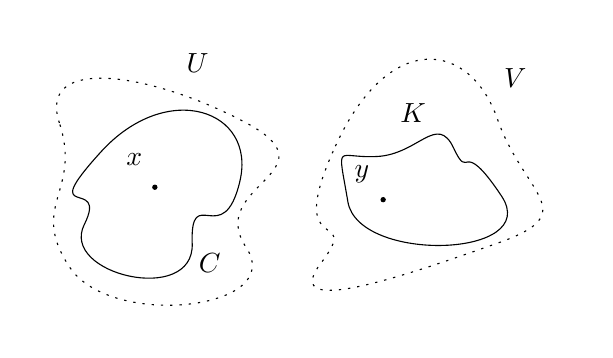
\begin{tikzpicture}[x=0.75pt,y=0.75pt,yscale=-1,xscale=1]
				%uncomment if require: \path (0,300); %set diagram left start at 0, and has height of 300
				
				%Shape: Circle [id:dp1732517118606005] 
				\draw  [fill={rgb, 255:red, 0; green, 0; blue, 0 }  ,fill opacity=1 ] (205,150) .. controls (205,149.45) and (205.45,149) .. (206,149) .. controls (206.55,149) and (207,149.45) .. (207,150) .. controls (207,150.55) and (206.55,151) .. (206,151) .. controls (205.45,151) and (205,150.55) .. (205,150) -- cycle ;
				%Shape: Polygon Curved [id:ds020722407137701016] 
				\draw  [dash pattern={on 0.84pt off 2.51pt}] (160,119) .. controls (149,85.6) and (206,95.4) .. (250,119) .. controls (294,142.6) and (230,149) .. (250,179) .. controls (270,209) and (185,218.6) .. (165,188.6) .. controls (145,158.6) and (171,152.4) .. (160,119) -- cycle ;
				%Shape: Circle [id:dp19705533391128083] 
				\draw  [fill={rgb, 255:red, 0; green, 0; blue, 0 }  ,fill opacity=1 ] (315,156) .. controls (315,155.45) and (315.45,155) .. (316,155) .. controls (316.55,155) and (317,155.45) .. (317,156) .. controls (317,156.55) and (316.55,157) .. (316,157) .. controls (315.45,157) and (315,156.55) .. (315,156) -- cycle ;
				%Shape: Polygon Curved [id:ds3453941623544552] 
				\draw  [dash pattern={on 0.84pt off 2.51pt}] (293,130.2) .. controls (319,73.4) and (358,79.8) .. (371,117) .. controls (384,154.2) and (413,162.2) .. (371,177) .. controls (329,191.8) and (265,214.2) .. (286,186.6) .. controls (307,159) and (267,187) .. (293,130.2) -- cycle ;
				%Shape: Polygon Curved [id:ds4009492428387247] 
				\draw   (180,133) .. controls (212,97.8) and (255,112.8) .. (247,147) .. controls (239,181.2) and (223,147.2) .. (224,177.2) .. controls (225,207.2) and (160,192) .. (172,168) .. controls (184,144) and (148,168.2) .. (180,133) -- cycle ;
				%Shape: Polygon Curved [id:ds362325771433208] 
				\draw   (313,135.2) .. controls (333,134.2) and (342,114.2) .. (350,131.2) .. controls (358,148.2) and (353,124.2) .. (373,154.2) .. controls (393,184.2) and (304,186.8) .. (299,157) .. controls (294,127.2) and (293,136.2) .. (313,135.2) -- cycle ;
				
				% Text Node
				\draw (191,132.4) node [anchor=north west][inner sep=0.75pt]    {$x$};
				% Text Node
				\draw (220,84.4) node [anchor=north west][inner sep=0.75pt]    {$U$};
				% Text Node
				\draw (301,138.4) node [anchor=north west][inner sep=0.75pt]    {$y$};
				% Text Node
				\draw (373,91.4) node [anchor=north west][inner sep=0.75pt]    {$V$};
				% Text Node
				\draw (226,180.6) node [anchor=north west][inner sep=0.75pt]    {$C$};
				% Text Node
				\draw (323,108.6) node [anchor=north west][inner sep=0.75pt]    {$K$};
				
				
			\end{tikzpicture}
		\end{center}
	\end{itemize}
\end{definizione}
\begin{lemma}\emph{\textbf{(di Urysohm)}}\index[analitico]{lemma!di Urysohm} Consideriamo $(X,\tau)$ uno spazio topologico. I seguenti fatti sono equivalenti:
	\begin{enumerate}[$(a)$]
		\item $(X,\tau)$ è normale,
		\item per ogni $C,K \subseteq X$ chiusi e disgiunti esiste  un'applicazione $f: X \to [0,1]$ continua tale che $f= 0$ su $C$ ed $f=1$ su $K$.
	\end{enumerate}
\end{lemma}
\begin{proof}
	Omettiamo la dimostrazione.
\end{proof}
\begin{osservazione}
	Il Lemma di Urysohm è considerato storicamente il primo risultato di topologia generale con una dimostrazione non banale: la difficoltà sta nelle ipotesi di lavoro molto generali. Se ci mettiamo però in un contesto metrico, basta considerare
	\[ f(x) = \frac{\textup{dist}(x,C)}{\textup{dist}(x,C)+ \textup{dist}(x,K)}. \]
\end{osservazione}
\begin{teorema}\emph{\textbf{(di Tietze)}}\index[analitico]{teorema!di Tietze}
	Consideriamo $(X,\tau)$ uno spazio topologico normale, $A \subseteq X$ chiuso e $f: A \to \R$ un'applicazione continua. Esiste un'applicazione $\tilde{f}: X \to \R$ continua tale che $\tilde{f}|_A = f$.
\end{teorema}
\begin{proof}
	Mostriamo innanzitutto che se esiste $C>0$ tale che, per ogni $x \in A$, $\abs{f(x)}\le C$, allora esiste un'applicazione $g:X\to \R$ continua tale che, per ogni $x \in X$, $\abs{g(x)}\le \frac{1}{3}C$ e, per ogni $x \in A$, $\abs{f(x)-g(x)}\le \frac{2}{3}C$. Siano $Y = f^{-1}([-C,-\frac{1}{3}C])$ $Z=f^{-1}([\frac{1}{3}C,C])$.
	\begin{center}
		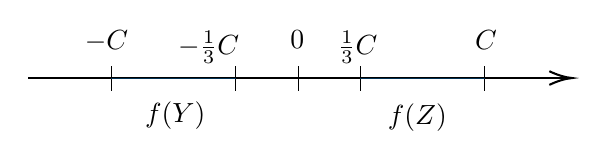
\begin{tikzpicture}[x=0.75pt,y=0.75pt,yscale=-1,xscale=1]
			%uncomment if require: \path (0,300); %set diagram left start at 0, and has height of 300
			
			%Straight Lines [id:da351590380041958] 
			\draw    (180,110.4) -- (440,110.4) ;
			\draw [shift={(442,110.4)}, rotate = 180] [color={rgb, 255:red, 0; green, 0; blue, 0 }  ][line width=0.75]    (10.93,-3.29) .. controls (6.95,-1.4) and (3.31,-0.3) .. (0,0) .. controls (3.31,0.3) and (6.95,1.4) .. (10.93,3.29)   ;
			%Straight Lines [id:da6689641897087604] 
			\draw    (310,104.6) -- (310,116.6) ;
			%Straight Lines [id:da03212271146730217] 
			\draw    (340,104.6) -- (340,116.6) ;
			%Straight Lines [id:da4012489765266216] 
			\draw    (400,104.6) -- (400,116.6) ;
			%Straight Lines [id:da5134778826508875] 
			\draw    (280,104.6) -- (280,116.6) ;
			%Straight Lines [id:da8281691966789628] 
			\draw    (220,104.6) -- (220,116.6) ;
			%Straight Lines [id:da30953233561890436] 
			\draw [color={rgb, 255:red, 0; green, 49; blue, 83 }  ,draw opacity=1 ][fill={rgb, 255:red, 0; green, 49; blue, 83 }  ,fill opacity=1 ]   (220,110.6) -- (280,110.6) ;
			%Straight Lines [id:da7267107874600898] 
			\draw [color={rgb, 255:red, 0; green, 49; blue, 83 }  ,draw opacity=1 ][fill={rgb, 255:red, 0; green, 49; blue, 83 }  ,fill opacity=1 ]   (340,110.6) -- (400,110.6) ;
			
			% Text Node
			\draw (305,86.4) node [anchor=north west][inner sep=0.75pt]    {$0$};
			% Text Node
			\draw (328,86.4) node [anchor=north west][inner sep=0.75pt]    {$\frac{1}{3} C$};
			% Text Node
			\draw (394,86.4) node [anchor=north west][inner sep=0.75pt]    {$C$};
			% Text Node
			\draw (251,86.4) node [anchor=north west][inner sep=0.75pt]    {$-\frac{1}{3} C$};
			% Text Node
			\draw (206,86.4) node [anchor=north west][inner sep=0.75pt]    {$-C$};
			% Text Node
			\draw (235,120.4) node [anchor=north west][inner sep=0.75pt]    {$f( Y)$};
			% Text Node
			\draw (352,121.4) node [anchor=north west][inner sep=0.75pt]    {$f( Z)$};
			
			
		\end{tikzpicture}
	\end{center}
	Siccome $f$ è continua, $Y$ e $Z$ sono chiusi in $A$, quindi lo sono in $X$, essendo $A$ chiuso. Sono inoltre disgiunti: infatti, se, per assurdo, esistesse $x \in Y \cap Z$, allora $f(x) \in [-C,-\frac{1}{3}C] \cap [\frac{1}{3}C,C] = \emptyset$, da cui la contraddizione. Per il Lemma di Urysohm, esiste $h: X \to [0,1]$ continua tale che $h=0$ su $Y$ e $h=1$ su $Z$. Mostriamo che $g: X \to \R$ tale che 
	\[ g(x) = \frac{2}{3}C\left( h(x)-\frac{1}{2}\right)  \]
	soddisfa i requisiti richiesti. In primo luogo, è chiaramente continua. Poi, per ogni $x \in X$
	\begin{align*}
		g(x) &\le  \frac{1}{3}C, & g(x) \ge - \frac{1}{3}C,
	\end{align*}
	quindi $\abs{g(x)}\le \frac{1}{3}C$. Ora, dal fatto che $A = Z \cup Y \cup f^{-1}([-\frac{C}{3},\frac{C}{3}])$, possiamo distinguere tre casi: se $x \in Y$, 
	\begin{align*}
		f(x) - g(x) &=  f(x) + \frac{1}{3}C \le 0 \le \frac{2}{3}C, & f(x) - g(x) \ge -C + \frac{1}{3}C = -\frac{2}{3}C;
	\end{align*}
	se $x \in Z$,
	\begin{align*}
		f(x) - g(x) &\le C - \frac{1}{3}C = \frac{2}{3}C, & f(x) - g(x) \ge \frac{1}{3}C - \frac{1}{3}C = 0 \ge -\frac{2}{3}C;
	\end{align*}
	se $x\in f^{-1}([-\frac{C}{3},\frac{C}{3}])$, ricordando che $h(x) \in [0,1]$,
	\begin{align*}
		f(x) - g(x) &\le \frac{C}{3} \le \frac{2}{3}C, & f(x) - g(x) \ge -\frac{2}{3}C.
	\end{align*}
	In ogni caso, $\abs{f(x)-g(x)}\le \frac{2}{3}C$. 
	
	Vediamo, dapprima, il caso $f:A \to [a,b]$, con $a<b \in \R$, continua. A meno di operare una traslazione ed un riscalamento, possiamo supporre $[a,b] = [0,1]$. Costruiamo ricorsivamente delle applicazioni $g_n: X \to \R$ continue tali che 
	\begin{align*}
		\forall\; x \in X: \;\abs{g_n(x)} &\le \frac{1}{3}\left( \frac{2}{3}\right) ^{n-1},\\
		\forall \; x \in A: \; \abs*{f(x)- \sum_{i=1}^{n}g_i(x)} &\le \left( \frac{2}{3}\right)^{n}.
	\end{align*}
	Siccome $\abs{f(x)}\le 1$ per ogni $x \in A$, l'esistenza di $g_1$ segue dal passaggio precedente. Supponiamo quindi di possedere $g_1,\dots,g_{n}$ e applichiamo il passaggio precedente a  
	\[ f_n =f- \sum_{i=1}^n g_i\]
	con $C = \left( \frac{2}{3}\right)^{n}$. Allora esiste $g_{n+1}: X \to \R$ continua tale che
	\begin{align*}
		\forall\; x \in X: \;\abs{g_{n+1}(x)} &\le \frac{1}{3}\left( \frac{2}{3}\right) ^{n},\\
		\forall \; x \in A: \; \abs*{f(x)- \sum_{i=1}^{n+1}g_i(x)} &\le \abs*{f(x)- \sum_{i=1}^{n}g_i(x) - g_{n+1}(x)} = \abs*{f_n(x)- g_{n+1}(x)}\le  \left( \frac{2}{3}\right)^{n+1}.
	\end{align*}
	Detta 
	\[ S_n(x) = \sum_{i=1}^{n}g_i(x), \]
	osserviamo che 
	\[ \sum_{i=1}^{\infty}\norm{g_i}_\infty \le \frac{1}{3} \sum_{i=1}^{\infty}\left( \frac{2}{3}\right)^{i-1} = 1, \]
	quindi la serie 
	\[ \sum_{i=1}^{\infty}g_i(x) \]
	è normalmente convergente in $C(X;\R)$, che è uno spazio di Banach. Allora esiste $\bar{f} \in  C(X;\R)$ tale che $S_n \to \bar{f}$ uniformemente\footnote{A voler essere precisi, dalla convergenza normale tiriamo fuori la convergenza uniforme e il limite uniforme di funzioni continue è continuo.}. Dal fatto che per ogni $x \in A$
	\[ \abs*{f(x)- \sum_{i=1}^{n}g_i(x)} \le \left( \frac{2}{3}\right)^{n}, \]
	segue che $\bar{f}|_A = f$. In particolare, per ogni $x \in X$,
	\[\bar{f}(x) \le \sum_{i=1}^{\infty}\norm{g_i}_\infty \le 1. \]
	A questo punto, basta considerare $\tilde{f} = (\bar{f})^+$. Chiaramente è una funzione continua. Poi, $0\le \tilde{f} \le 1$ e, su $ A$, $\bar{f}=f$, quindi $\tilde{f} = f^+ = f$, essendo $f\ge 0$, e possiamo concludere che $\tilde{f}$ soddisfa i requisiti richiesti.
	
	Vediamo, poi, il caso $f:A \to \left] -1,1\right[ $ continua. Siccome $\left] -1,1\right[ \subseteq [-1,1]$, dal passaggio precedente, esiste $\overline{f}: X \to [-1,1]$ tale che $\overline{f}|_A = f$. Sia $B= \overline{f}^{-1}(\left\lbrace -1,1\right\rbrace )$, chiuso in $X$ perché $\overline{f}$ continua e $A$ chiuso. Siccome $f$ è a valori in $\left] -1,1\right[$, allora $A \cap B = \emptyset$, quindi per il Lemma di Urysohm, esiste $k : X \to [0,1]$ tale che $k=1$ in $A$ e $k=0$ in $B$. Vediamo che l'applicazione $\tilde{f} = k\overline{f}: X \to \left] -1,1\right[$ soddisfa i requisiti richiesti. Innanzitutto, se $\overline{f}(x) \in \left] -1,1\right[ $, allora $\tilde{f} \in \left] -1,1\right[$. Invece, se $\overline{f}(x) \in \left\lbrace -1,1\right\rbrace$, $\tilde{f}(x) = 0 \in \left] -1,1\right[$, in quanto $k=0$ in $B$. In particolare, $\tilde{f}$ è ben definita. Chiaramente è poi continua e $\tilde{f}|_A = f$, in quanto $k = 1$ in $A$.
	
	Nel caso generale, sia $\Phi: \R \to \left] -1,1\right[$ un omeomorfismo.\footnote{Possiamo, ad esempio, prendere $\Phi^{-1}:\left] -1,1\right[ \to \R$ tale che
		\[ \Phi^{-1}(x)= \begin{cases}
			\frac{x}{x+1} & \textup{se } -1<x\le 0,\\
			\frac{x}{1-x} & \textup{se } 0\le x< 1,\\
		\end{cases} \]
		oppure un opportuno riscalamento della funzione $\arctan$.
	} Applicando il caso precedente a  $ \Phi\circ f: A \to \left] -1,1\right[$, segue l'esistenza di $\overline{f}: X \to \left] -1,1\right[$ tale che $\overline{f}|_A = \Phi\circ f$. A questo punto basta considerare $\tilde{f} = \Phi^{-1}\circ \overline{f}$.
\end{proof}

\begin{teorema}\textbf{\emph{(di invarianza del dominio)}}\index[analitico]{teorema!di invarianza!del dominio}
	Sia $U \subseteq \R^n$ aperto. Se $f: U \to \R^n$ è un'applicazione iniettiva e continua, allora $f(U)$ è aperto. In particolare, $f: U \to f(U)$ è un omeomorfismo.
\end{teorema}
\begin{proof}
	È sufficiente dimostrare che se  $f: \overline{\B(0,1)} \to \R^n$ è un'applicazione iniettiva e continua, allora $f(0) \in \textup{int}(f(\overline{\B(0,1)}))$. Infatti, la tesi corrisponde a richiedere che
	\[ y \in f(U) \Longrightarrow y \in \textup{int}(f(U)), \]
	ossia
	\[ x_0 \in U \Longrightarrow f(x_0) \in \textup{int}(f(U)), \]
	ma, a meno di una traslazione, possiamo sempre supporre che $x_0=0$, quindi la tesi sarebbe
	\[ f(0) \in \textup{int}(f(U)). \]
	Ora, siccome $U$ è aperto, a meno di un riscalamento, $0 \in \overline{\B(0,1)}\subsetneq U$. %Se $f(x) \in f(\overline{\B(0,1)})$, allora $x \in \overline{\B(0,1)}$, quindi $x \in U$, allora $f(x) \in f(U)$: in altre parole $f(\overline{\B(0,1)}) \subseteq f(U)$. In particolare, $f(\overline{\B(0,1)}) \subsetneq f(U)$: supponiamo, per assurdo, che  $f(\overline{\B(0,1)}) = f(U)$. Siccome $\overline{\B(0,1)}\subsetneq U$, esiste $\xi \in U \setminus \overline{\B(0,1)}$, ma, per ipotesi assurda, trovo anche $\eta \in \overline{\B(0,1)}$ tale che $f(\eta) = f(\xi)$. Dovendo essere, $\xi \ne \eta$, l'assurdo deriva dalla violazione dell'iniettività di $f$. 
	In particolare, siccome, per iniettività, $f(\overline{\B(0,1)}) \subseteq f(U)$, è sufficiente dimostrare che $f(0) \in \textup{int}(f(\overline{\B(0,1)}))$ e possiamo anche pensare direttamente che $f: \overline{\B(0,1)} \to \R^n$.
	
	Supponiamo, per assurdo che $f(0) \notin \textup{int}(f(\overline{\B(0,1)}))$. Allora, deve essere $f(0) \in \partial (f(\overline{\B(0,1)}))$, perché $f(0) \in f(\overline{\B(0,1)})$. In particolare, per ogni $\varepsilon > 0$, esiste $c \in \R^n\setminus f(\overline{\B(0,1)})$ tale che $\abs{c-f(0)}<\varepsilon$. Detti 
	\begin{align*}
		\Sigma_1 &= \left\lbrace y \in f(\overline{\B(0,1)}): \abs{y-c}\ge \varepsilon\right\rbrace,\\
		\Sigma_2 &= \left\lbrace y \in \R^n: \abs{y-c}= \varepsilon\right\rbrace,
	\end{align*}
	consideriamo l'insieme $\Sigma = \Sigma_1 \cup \Sigma_2$: in primo luogo $\Sigma_1$ è chiuso in $f(\overline{\B(0,1)})$\footnote{Perchè il suo complementare è l'intersezione di $f(\overline{\B(0,1)})$ con la palla aperta $\B(c,\varepsilon)$.}, che è compatto, siccome $f$ è continua, quindi $\Sigma_1$ è compatto. Poi $\Sigma_2 = \partial \B(c,\varepsilon)$, quindi anche lui è compatto. Essendo $\Sigma$ l'unione di due compatti, è anch'esso compatto. In più, $f(0) \notin \Sigma$.
	
	\begin{center}
		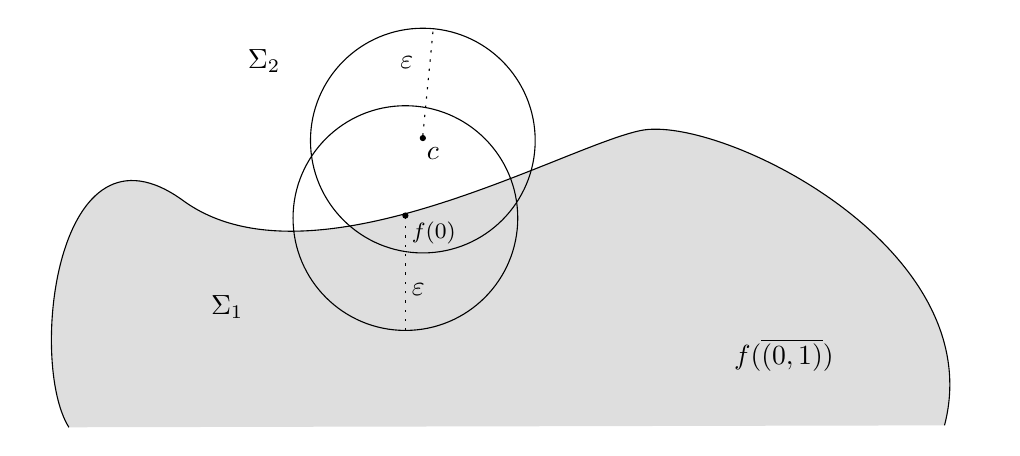
\begin{tikzpicture}[x=0.70pt,y=0.70pt,yscale=-1,xscale=1]
			%uncomment if require: \path (0,300); %set diagram left start at 0, and has height of 300
			
			%Curve Lines [id:da21018532107485988] 
			\draw [fill={rgb, 255:red, 155; green, 155; blue, 155 }  ,fill opacity=0.33 ]   (122,244.6) .. controls (101,211.6) and (115,79.6) .. (181,127.6) .. controls (247,175.6) and (377,99.6) .. (417.28,91.38) .. controls (457.56,83.16) and (598,151.6) .. (574,243.6) ;
			%Shape: Circle [id:dp004821536589640019] 
			\draw  [fill={rgb, 255:red, 0; green, 0; blue, 0 }  ,fill opacity=1 ] (294.4,135.3) .. controls (294.4,134.58) and (294.98,134) .. (295.7,134) .. controls (296.42,134) and (297,134.58) .. (297,135.3) .. controls (297,136.02) and (296.42,136.6) .. (295.7,136.6) .. controls (294.98,136.6) and (294.4,136.02) .. (294.4,135.3) -- cycle ;
			%Shape: Circle [id:dp8290836366492667] 
			\draw   (237.7,136.6) .. controls (237.7,104.57) and (263.67,78.6) .. (295.7,78.6) .. controls (327.73,78.6) and (353.7,104.57) .. (353.7,136.6) .. controls (353.7,168.63) and (327.73,194.6) .. (295.7,194.6) .. controls (263.67,194.6) and (237.7,168.63) .. (237.7,136.6) -- cycle ;
			%Shape: Circle [id:dp2809219934901368] 
			\draw  [fill={rgb, 255:red, 0; green, 0; blue, 0 }  ,fill opacity=1 ] (303.4,95.3) .. controls (303.4,94.58) and (303.98,94) .. (304.7,94) .. controls (305.42,94) and (306,94.58) .. (306,95.3) .. controls (306,96.02) and (305.42,96.6) .. (304.7,96.6) .. controls (303.98,96.6) and (303.4,96.02) .. (303.4,95.3) -- cycle ;
			%Shape: Circle [id:dp9678593963925135] 
			\draw   (246.7,96.6) .. controls (246.7,64.57) and (272.67,38.6) .. (304.7,38.6) .. controls (336.73,38.6) and (362.7,64.57) .. (362.7,96.6) .. controls (362.7,128.63) and (336.73,154.6) .. (304.7,154.6) .. controls (272.67,154.6) and (246.7,128.63) .. (246.7,96.6) -- cycle ;
			%Straight Lines [id:da42967896812356576] 
			\draw  [dash pattern={on 0.84pt off 2.51pt}]  (295.7,194.6) -- (295.7,136.6) ;
			%Straight Lines [id:da2746572242277334] 
			\draw  [dash pattern={on 0.84pt off 2.51pt}]  (304.7,94) -- (310,39.6) ;
			
			% Text Node
			\draw (297.7,137.4) node [anchor=north west][inner sep=0.75pt]  [font=\footnotesize]  {$f( 0)$};
			% Text Node
			\draw (194,175.4) node [anchor=north west][inner sep=0.75pt]    {$\Sigma _{1}$};
			% Text Node
			\draw (464,197.4) node [anchor=north west][inner sep=0.75pt]    {$f(\overline{\B(0,1)})$};
			% Text Node
			\draw (305.4,98.7) node [anchor=north west][inner sep=0.75pt]    {$c$};
			% Text Node
			\draw (297.7,169) node [anchor=north west][inner sep=0.75pt]    {$\varepsilon $};
			% Text Node
			\draw (291.7,52) node [anchor=north west][inner sep=0.75pt]    {$\varepsilon $};
			% Text Node
			\draw (213,48.4) node [anchor=north west][inner sep=0.75pt]    {$\Sigma _{2}$};
		\end{tikzpicture}
	\end{center}
	
	Mostriamo che $f: \overline{\B(0,1)} \to f(\overline{\B(0,1)})$ è un omeomorfismo. Chiaramente è biettiva, quindi basta mostrare che $f^{-1}:f(\overline{\B(0,1)}) \to \overline{\B(0,1)}$ è continua. Siano quindi $y \in f(\overline{\B(0,1)})$ e $(y_h)$ in $f(\overline{\B(0,1)})$ tali che $y_h \to y$. Data $(f^{-1}(y_h))$, consideriamo una qualsiasi sua sottosuccessione $(f^{-1}(y_{h_k}))$. Sia $(x_{h_k})$ in $\overline{\B(0,1)}$ tale che $y_{h_k} = f(x_{h_k})$. Per compattezza, esistono $x \in \overline{\B(0,1)}$ e $(x_{h_{k_j}})$ tali che $x_{h_{k_j}} \to x$. Essendo $f$ continua, allora $f(x_{h_{k_j}}) \to f(x)$, ossia $y_{h_{k_j}} \to f(x)$ e, per unicità del limite, $y = f(x)$ o, in altre parole, $x = f^{-1}(y)$. Quindi $f^{-1}(y_{h_{k_j}}) \to f^{-1}(y)$. Allora $f^{-1}(y_h)\to f^{-1}(y)$, quindi $f^{-1}$ è continua.
	
	A questo punto, essendo, per la continuità di $f$, $f(\overline{\B(0,1)})$ compatto, quindi completo, quindi chiuso, per il Teorema di Tietze, applicato componente per componente, esiste un'applicazione $g: \R^n \to \R^n$ continua tale che $g = f^{-1}$ su $f(\overline{\B(0,1)})$. 
	
	Osserviamo che $g \ne 0$ su $\Sigma_1$: infatti se, per assurdo, esiste $y \in \Sigma_1 \subseteq f(\overline{\B(0,1)})$ tale che $g(y)=0$, allora esiste $x \in \overline{\B(0,1)}$ tale che $y=f(x)$, ma $0= g(y) = f^{-1}(y) = x$, ossia $y = f(0) \in \Sigma_1$, assurdo. Quindi, per la compattezza di $\Sigma_1$ e la continuità di $g$, esiste $\delta >0$, che, senza perdita di generalità, possiamo supporre $\delta < \frac{1}{2}$, tale che per ogni $y \in \Sigma_1$
	\[ \abs{g(y)} \ge \delta. \]
	Per il Teorema di Stone--Weierstrass, essendo $\Sigma$ compatto, esiste un'applicazione a componenti polinomiali $p:\R^n \to \R^n$ tale che per ogni $y \in \Sigma$
	\[ \abs{p(y)-g(y)}< \frac{\delta}{2}. \]
	Osserviamo che $p \ne 0$ su $\Sigma_1$\footnote{Potrebbe però annullarsi su $\Sigma_2$.}: se così non fosse, esisterebbe $y \in \Sigma_1$ tale che $\abs{g(y)}<\frac{\delta}{2}$, assurdo.
	
	Mostriamo che esiste $a_0 \in \B(0,\frac{\delta}{2})\setminus p(\Sigma_2)$. Innanzitutto, $p$ ha componenti polinomiali, quindi è almeno di classe $C^1$. In particolare, $p$ è lipschitziana su $\B(c,2\varepsilon)$ con costante di Lipschitz $A$. Allora,
	\[ \mathcal{L}^n(p(\Sigma_2))\le A^n \mathcal{L}^n(\Sigma_2) =0. \]
	Se, per assurdo, per ogni $a \in \B(0,\frac{\delta}{2})$ si avesse $a \in p(\Sigma_2)$, allora $\B(0,\frac{\delta}{2}) \subseteq p(\Sigma_2)$, quindi, per la monotonia della misura di Lebesgue,
	\[ \mathcal{L}^n(\B(0,\frac{\delta}{2})) \le \mathcal{L}^n(p(\Sigma_2)) = 0, \]
	assurdo.
	
	Poniamo $\tilde{p} = p - a_0$. Osserviamo che $\tilde{p} \ne 0$ su $\Sigma$: innanzitutto, per ogni $y \in \Sigma$
	\[ \abs{\tilde{p}(y)-g(y)} \le \abs{p(y)-g(y)} + \abs{a_0} < \delta, \]
	quindi, come sopra, $\tilde{p} \ne 0$ su $\Sigma_1$. Inoltre, se, per assurdo, esistesse $y \in \Sigma_2$ tale che $\tilde{p}(y) = 0$, allora avremmo $a_0 = p(y) \in p(\Sigma_2)$, assurdo.
	
	Consideriamo $\Phi: f(\overline{\B(0,1)}) \to \Sigma$ tale che
	\[ f(y) = \begin{cases}
		y & \textup{se } \abs{y-c}\ge \varepsilon,\\
		c + \varepsilon \frac{y-c}{\abs{y-c}} & \textup{se } \abs{y-c}<\varepsilon.
	\end{cases} \]
	Anzitutto, $\Phi$ è ben definita: $c \notin f(\overline{\B(0,1)})$, quindi il denominatore non si annulla mai; inoltre, se $\abs{y-c} \ge \varepsilon$, $\Phi(y) = y \in \Sigma_1 \subseteq \Sigma$ mentre se $\abs{y-c} < \varepsilon$, allora 
	\[ \abs{\Phi(y)-c} = \varepsilon,\]
	quindi $\Phi(y) \in \Sigma_2 \subseteq \Sigma$. In più, $\Phi$ è continua: se $\abs{y-c} = \varepsilon$, allora
	\[ c + \varepsilon \frac{y-c}{\abs{y-c}} = c + y - c = y. \]
	
	Presa $h = \tilde{p} \circ \Phi: f(\overline{\B(0,1)}) \to \R^n$, continua per composizione, si ha che $h \ne 0$. Mostriamo che per ogni $x \in \overline{\B(0,1)}$ 
	\[ \abs{h(f(x))-x}\le 1. \]
	Per continuità di $g$ in $f(0)$, scegliamo $\varepsilon$ tale che
	\[ \abs{y - f(0)} < 2\varepsilon \Longrightarrow \abs{g(y)} = \abs{g(y)-g(f(0))} <\frac{1}{4}. \]
	Distinguiamo due casi: se $f(x) \in \Sigma_1$, 
	\[ \abs{h(f(x))-x} = \abs{\tilde{p}(\Phi(f(x))) -x} = \abs{\tilde{p}(f(x))-x} = \abs{\tilde{p}(f(x))- g(f(x))} < \delta < \frac{1}{2}<1. \]
	Se, invece, $y = f(x) \notin \Sigma_1$, allora $\abs{y-c}<\varepsilon$, quindi 
	\[ \abs{y - f(0)} \le \abs{y-c}+\abs{c-f(0)} < 2\varepsilon, \] 
	da cui $\abs{g(y)}<\frac{1}{4}$. Inoltre, 
	\[ \abs{\Phi(y) - f(0)} \le \abs{\Phi(y)-c}+\abs{c-f(0)} < 2\varepsilon, \] 
	da cui $\abs{g(\Phi(y))}<\frac{1}{4}$. Perciò,
	\begin{align*}
		\abs{h(f(x))-x} &= \abs{h(y) -g(y)} \le \abs{\tilde{p}(\Phi(y)))-g(\Phi(y))} + \abs{g(\Phi(y)) - g(y)} < \\
		&< \delta + \abs{g(\Phi(y)) } +\abs{g(y)}< 1.
	\end{align*}
	
	A questo punto, detta $\tilde{h}:\overline{\B(0,1)} \to \R^n$ tale che
	\[ \tilde{h}(x) = x-h(f(x)), \]
	chiaramente continua, si ha che, per ogni $x \in  \overline{\B(0,1)}$, $\abs{\tilde{h}(x)}\le 1$, ossia $\textup{Im}(\tilde{h})\subseteq \overline{\B(0,1)}$. Per il Teorema di Brouwer, esiste quindi $x_0 \in \overline{\B(0,1)}$ tale che $\tilde{h}(x_0) = x_0$, ossia $h(f(x_0)) = 0$, assurdo e la dimostrazione è conclusa.
\end{proof}
Per comprendere l'importanza delle ipotesi del Teorema di invarianza del dominio vediamo due controesempi evocativi.
\begin{esempio}
	Consideriamo l'applicazione continua e iniettiva $f: \left] 0,1\right[ \to \R^2$ tale che
	\[ f(t) = (t,0). \]
	Siccome $ \left] 0,1\right[ \subseteq \R$ e $1 \ne 2$, il Teorema di invarianza del dominio non si applica. Ciò accade a buon titolo, infatti $f( \left] 0,1\right[) =  \left] 0,1\right[ \times \left\lbrace 0\right\rbrace$, che non è aperto in $\R^2$.
\end{esempio}

\begin{esempio}
	Consideriamo l'applicazione continua e iniettiva $T_r: l^2(\R) \to l^2(\R) $ tale che
	\[ T_r((a_n)) = (0,a_0,a_1,a_2,\dots). \]
	Siccome $ l^2(\R) $ non ha dimensione finita, il Teorema di invarianza del dominio non si applica. Ciò accade a buon titolo, infatti $T_r(l^2(\R))$ non è aperto. Se per assurdo lo fosse, per ogni $(b_n) \in T_r(l^2(\R))$, ossia
	\[ (b_n) = (0,b_1,b_2,\dots), \]
	esisterebbe $r >0$ tale che $B((b_n),r) \subseteq T_r(l^2(\R))$. Ma ciò è assurdo perché 
	\[ (c_n) = \left( \frac{r}{2},b_1,b_2,\dots\right)  \in B((b_n),r),\]
	in quanto $\norm{(c_n)-(b_n)}_{l^2(\R)} = \frac{r}{2}<r$, ma $c_0 = \frac{r}{2} \ne 0$, quindi $(c_n) \in l^2(\R) \setminus T_r(l^2(\R))$.
\end{esempio}
Una conseguenza diretta del Teorema di invarianza del dominio è il seguente risultato.
\begin{teorema}\textbf{\emph{(di invarianza della dimensione)}}\index[analitico]{teorema!di invarianza!della dimensione}
	Siano $U \subseteq \R^n$ e $V \subseteq \R^m$ aperti. Se $n \ne m$, allora $U$ non è omeomorfo a $V$. In particolare, $\R^n$ non è omeomorfo a $\R^m$.
\end{teorema}
\begin{proof}
	Senza perdita di generalità, supponiamo $m > n$. Sia $i: \R^n \to \R^m$ tale che
	\[ i(x) = (x_1,\dots,x_n,0,\dots,0). \]
	Supponiamo, per assurdo, che esista un omeomorfismo $f: V \to U$ e consideriamo $g = i \circ f: V \to \R^m$. Chiaramente $g$ è continua e, dati $x,y \in V $ tali che $g(x) = g(y)$, risulta
	\[ (f_1(x),\dots,f_n(x),0,\dots,0) = (f_1(y),\dots,f_n(y),0,\dots,0). \]
	In particolare, $f(x) = f(y)$ che, essendo $f$ un omeomorfismo, quindi iniettiva, conduce a $x=y$. In altre parole $g$ è pure iniettiva. Per il Teorema di invarianza del dominio, $g(V)$ è aperto in $\R^m$, quindi per ogni $y \in g(V)$ esiste $r>0$ tale che $B(y,r) \subseteq g(V)$. Ma ciò è assurdo perché $z = \left( y_1,\dots,y_n,\frac{r}{2},0,\dots,0\right)  \in B(y,r)$, ma $z \in \R^m \setminus g(V)$.
\end{proof}

Grazie al Teorema di Brouwer è anche possibile dare una dimostrazione alternativa del Teorema fondamentale dell'Algebra.
\begin{teorema}\textbf{\emph{(fondamentale dell'Algebra)}}\index[analitico]{teorema!fondamentale dell'Algebra}
	Sia 
	\[ P(z) = \sum_{k=0}^{n}a_kz^k \]
	una funzione polinomiale complessa con $n\ge 1$ ed $a_n \ne 0$. Allora esiste $z \in \C$ tale che $P(z) = 0$.
\end{teorema}
\begin{proof}
	Innanzitutto, senza perdita di generalità, possiamo supporre $a_n = 1$ e identificare $\C$ con $\R^2$. Sia $r = 2 + \displaystyle\sum_{k=0}^{n-1}\abs{a_k}$ e $g: \overline{\B(0,r)} \to \C$ tale che
	\[ g(z) = \begin{cases}
		z- \frac{P(z)}{r}e^{i(1-n)\vartheta} & \textup{se } \abs{z} \le 1,\\
		z- \frac{P(z)}{r}z^{(1-n)} & \textup{se } \abs{z} > 1,
	\end{cases} \]
	ben definita e continua in quanto se $\abs{z} = 1$, $z = e^{i\vartheta}$ per qualche $\vartheta$ e $e^{i(1-n)\vartheta} = (e^{i\vartheta})^{1-n}$. Mostriamo che $\textup{Im}(g) \subseteq \overline{\B(0,r)}$. Se $\abs{z} \le 1$, 
	\[ \abs{g(z)} \le \abs{z} + \frac{\abs{P(z)}}{r} \le 1 + \frac{1+ \displaystyle\sum_{k=0}^{n-1}\abs{a_k}}{2+ \displaystyle\sum_{k=0}^{n-1}\abs{a_k}} \le 1+ 1 = 2 \le r.\]
	Se, invece, $1<\abs{z}\le r$, allora
	\[ \abs{g(z)} = \abs*{z - \frac{z}{r} - \frac{1}{rz^{n-1}}\sum_{k=0}^{n-1}a_kz^k} = \abs*{\frac{r-1}{r}z -\frac{1}{rz^{n-1}}\sum_{k=0}^{n-1}a_kz^k} \le \frac{r-1}{r}\abs{z} + \sum_{k=0}^{n-1}\frac{\abs{a_k}\abs{z^k}}{r\abs{z}^{n-1}},\]
	quindi 
	\[ \abs{g(z)} \le r-1 + \sum_{k=0}^{n-1}\frac{\abs{a_k}}{r\abs{z}^{n-1-k}} \le r-1 + \frac{\displaystyle\sum_{k=0}^{n-1}\abs{a_k}}{r} \le r-1 + 1 = r.\]
	
	Da ciò, per il Teorema di Brouwer, esiste $z \in \overline{\B(0,r)} \subseteq \C$ tale che $g(z) = z$, ossia $P(z) = 0$, che è la tesi.
\end{proof}

\section{Risultati in dimensione infinita}
Passiamo invece ai risultati che valgono senza l'ipotesi di dimensione finita.
\begin{teorema}\emph{\textbf{(di Schauder)}}\index[analitico]{teorema!di Schauder}
	Consideriamo $(X,\norm{\;})$ uno spazio normato su $\R$. Siano $C \subseteq X$ convesso, chiuso, limitato e non vuoto
	ed un'applicazione $f: C \to C$ continua e compatta. Esiste $x \in C$ tale che $f(x) = x$.
\end{teorema}
\begin{proof}
	Omettiamo la dimostrazione.
\end{proof}
Vediamo subito un'applicazione del Teorema di Schauder.
\begin{teorema}\textbf{\emph{(di Peano)}}\index[analitico]{teorema!di Peano}
	Siano $ (t_{0},u_{0}) \in \R\times\R^{n}$, $ a,b,r >0 $ e  
	\[ f: \left[t_{0} - a,t_{0}+b\right] \times \overline{\textup{B}(u_{0},r)} \to \R^{n} \]
	una applicazione continua tale che 
	\[ (b-a)\max\left\lbrace \abs*{f(\tau,\xi)} \; : \; \tau \in \left[t_{0} - a,t_{0} +b\right], \; \xi \in \overline{\textup{B}(u_{0},r)}\right\rbrace \le r. \]
	Allora esiste 
	\[ u: \left[t_{0} - a,t_{0}+b\right] \to \R^{n}, \]
	una soluzione del problema di Cauchy
	\[ \begin{cases}
		u' = f(t,u), \\
		u(t_{0}) = u_{0}.
	\end{cases} \]
\end{teorema}
\begin{proof}
	Essendo $f$ continua, $u: \left[t_{0} - a,t_{0}+b\right] \to \R^{n}$ è soluzione del problema di Cauchy \[ \begin{cases}
		u' = f(t,u), \\
		u(t_{0}) = u_{0},
	\end{cases} \]
	se e solo se $u$ è continua e per ogni $t \in \left[t_{0} - a,t_{0}+b\right]$
	\[ u(t) = u_0 + \int_{t_0}^{t} f(\tau,u(\tau)) d\tau.\]
	Per ogni $u \in \overline{\B(u_0,r)} \subseteq C(\left[t_{0} - a,t_{0}+b\right];\R^n)$ consideriamo il funzionale
	\[ \Phi(u)(t) = u_0 + \int_{t_0}^{t} f(\tau,u(\tau)) d\tau. \]
	Osserviamo che 
	\begin{align*}
		\abs{\Phi(u)(t) - u_0} \le\int_{t_0}^{t}\abs{f(\tau,u(\tau))d\tau}\le \frac{r}{b-a}(b-a) = r,
	\end{align*}
	per cui $\norm{\Phi(u) - u_0}_\infty \le r$. In altre parole possiamo pensare che $\Phi:\overline{\B(u_0,r)} \to \overline{\B(u_0,r)}$. La continuità di $\Phi$ discende dal Teorema della convergenza dominata, mostriamo quindi che $\Phi$ è compatto. Sia $(u_h)$ in $\overline{\B(u_0,r)}$, chiaramente limitata. Siccome $\textup{Im}(\Phi) \subseteq \overline{\B(u_0,r)}$, chiaramente $(\Phi(u_h))$ è limitata. Dato $\varepsilon > 0$, sia $\delta = \frac{\varepsilon(b-a)}{r}$. Allora per ogni $h \in \N$ e per ogni $s,t \in \left[t_{0} - a,t_{0}+b\right]$ tali che $\abs{t-s} < \delta$
	\[ \abs{\Phi(u_h)(t) - \Phi(u_h)(s)} \le \abs*{\int_{s}^{t}\abs{f(\tau,u_h(\tau))}d\tau} \le \frac{r}{b-a}\abs{t-s} < \varepsilon.\]
	Per il Teorema di Ascoli--Arzelà, esiste una sottosuccessione $(u_{h_k})$ convergente, ossia $\Phi$ è compatto. 
	
	Dal Teorema di Schauder discende quindi che esiste $u \in \overline{\B(u_0,r)}$ tale che $\Phi(u) = u$, da cui la tesi.
\end{proof}

Il risultato gemello del Teorema di Schauder è il seguente.
\begin{teorema}\emph{\textbf{(di Tychonoff)}}\index[analitico]{teorema!di Tychonoff}
	Consideriamo $(X,\norm{\;})$ uno spazio normato su $\R$. Siano $K \subseteq X$ convesso, compatto e non vuoto ed un'applicazione $f : K \to K$ continua. Esiste $x \in K$ tale che $f(x) = x$.
\end{teorema}
\begin{proof}
	Innanzitutto, fissato $\varepsilon>0$,
	\[ \bigcup_{x \in K}B(x,\varepsilon) \]
	è un ricoprimento aperto di $K$. Per compattezza, esistono quindi $x_1,\dots,x_{n_\varepsilon} \in K$ tali che
	\[ K \subseteq \bigcup_{i=1}^{n_\varepsilon}\B(x_i,\varepsilon). \]
	Consideriamo l'inviluppo convesso chiuso di $x_1,\dots, x_{n_\varepsilon}$, ossia
	\[ K_\varepsilon = \left\lbrace \sum_{i=1}^{n_\varepsilon} \lambda_i x_i : \lambda_i \in [0,1], \sum_{i=1}^{n_\varepsilon} \lambda_i =1\right\rbrace. \]
	
	Osserviamo che $K_\varepsilon$ è chiuso e convesso. Sia $\sum_{i=1}^{n_\varepsilon}\lambda_i^{(h)}x_i \to y \in X$. La successione $((\lambda_1^{(h)},\dots,\lambda_{n_\varepsilon}^{(h)}))$ è limitata in $[0,1]^{n_\varepsilon}$ quindi, per il Teorema di Bolzano--Weierstrass ed il fatto che  $[0,1]^{n_\varepsilon}$ è chiuso in $\R^{n_\varepsilon}$, esiste $(\lambda_1,\dots,\lambda_{n_\varepsilon}) \in [0,1]^{n_\varepsilon}$ tale che, a meno di sottosuccessioni, $(\lambda_1^{(h)},\dots,\lambda_{n_\varepsilon}^{(h)}) \to (\lambda_1,\dots,\lambda_{n_\varepsilon})$ in $\R^{n_\varepsilon}$. Passando al limite in 
	\[ \sum_{i=1}^{n_\varepsilon}\lambda_i^{(h_k)} = 1, \]
	otteniamo anche che 
	\[ \sum_{i=1}^{n_\varepsilon}\lambda_i = 1. \]
	In particolare poi, per continuità delle operazioni di somma e prodotto per scalare, 
	\[ \sum_{i=1}^{n_\varepsilon}\lambda_i^{(h_k)}x_i \to \sum_{i=1}^{n_\varepsilon}\lambda_ix_i,  \]
	quindi per unicità del limite deve essere $y = \displaystyle\sum_{i=1}^{n_\varepsilon}\lambda_ix_i \in K_\varepsilon$, da cui la chiusura di $K_\varepsilon$. Per quanto riguarda la convessità invece, se $\displaystyle\sum_{i=1}^{n_\varepsilon}\lambda_i x_i, \displaystyle\sum_{i=1}^{n_\varepsilon}\overline{\lambda}_i x_i \in K_\varepsilon$ e $\lambda \in [0,1]$
	\[ \lambda \sum_{i=1}^{n_\varepsilon}\lambda_i x_i + (1-\lambda)\sum_{i=1}^{n_\varepsilon}\overline{\lambda}_i x_i =  \sum_{i=1}^{n_\varepsilon}[\lambda \lambda_i +(1-\lambda)\overline{\lambda}_i]x_i \in K_\varepsilon  \]
	siccome, per convessità di $[0,1]$, per ogni $i=1,\dots,n_{\varepsilon}$ si ha che $\lambda \lambda_i +(1-\lambda)\overline{\lambda}_i \in [0,1]$ e 
	\[ \sum_{i=1}^{n_\varepsilon}\left( \lambda \lambda_i +(1-\lambda)\overline{\lambda}_i\right) = \lambda  \sum_{i=1}^{n_\varepsilon} \lambda_i +(1-\lambda) \sum_{i=1}^{n_\varepsilon}\overline{\lambda}_i = \lambda + 1 -\lambda = 1. \]
	
	Mostriamo che $K_\varepsilon \subseteq K$. Chiaramente, per ogni $i= 1,\dots, n_\varepsilon$ si ha $x_i \in K$. Poi, essendo $K$ convesso, per ogni $i,j = 1,\dots,n_\varepsilon$, dato $\lambda_i \in [0,1]$, si ha $\lambda_ix_i +(1-\lambda_i)x_j \in K$. Ora, per ogni $i,j,k=1,\dots,n_\varepsilon$, consideriamo $\lambda_i,\lambda_j,\lambda_k \in [0,1]$ tali che $\lambda_i + \lambda_j + \lambda_k = 1$. Preso
	\[ y = \frac{\lambda_j}{\lambda_j + \lambda_k}x_j + \frac{\lambda_k}{\lambda_j + \lambda_k}x_k, \]
	dal fatto che 
	\begin{align*}
		\frac{\lambda_k}{\lambda_j + \lambda_k} &\in [0,1], & \frac{\lambda_k}{\lambda_j + \lambda_k} &= 1 - \frac{\lambda_j}{\lambda_j + \lambda_k}
	\end{align*}
	e dal passo precedente, segue che $y \in K$. In particolare, 
	\[ \lambda_i x_i + \lambda_j x_j + \lambda_k x_k = \lambda_i x_i + (1-\lambda_i)y \in K.\]
	Procedendo ricorsivamente, si ottiene $K_\varepsilon \subseteq K$. In particolare, essendo $K_\varepsilon$ chiuso in un compatto, è anch'esso compatto.
	
	Consideriamo ora $P_\varepsilon : K \to K_\varepsilon$ tale che
	\[ P_\varepsilon(x) = \dfrac{\displaystyle \sum_{i=1}^{n_\varepsilon}\textup{dist}(x,K\setminus \B(x_i,\varepsilon))x_i}{\displaystyle\sum_{i=1}^{n_\varepsilon}\textup{dist}(u,K\setminus \B(x_i,\varepsilon))}. \]
	Vediamo che è ben definita. Innanzitutto, il denominatore è sempre diverso da zero: infatti, essendo una somma di termini positivi, per essere nullo dovrebbe avere tutti gli addendi nulli e, se ciò si verificasse, per ogni $i=1,\dots,n_\varepsilon$ si avrebbe $x \in K\setminus \B(x_i,\varepsilon)$, ossia $x \notin \B(x_i,\varepsilon)$, che contraddirebbe il fatto che K è ricoperto dall'unione delle $\B(x_i,\varepsilon)$. Inoltre, per ogni $i=1,\dots,n_\varepsilon$ si ha
	\begin{align*}
		\lambda_i = \dfrac{\textup{dist}(x,K\setminus \B(x_i,\varepsilon))}{\displaystyle\sum_{i=1}^{n_\varepsilon}\textup{dist}(x,K\setminus \B(x_i,\varepsilon))} &\in [0,1], & \sum_{i=1}^{n_{\varepsilon}}\lambda_i &= 1, 
	\end{align*}
	quindi $P_\varepsilon(x) \in K_\varepsilon$. In più, $P_\varepsilon$ è continua per costruzione e per ogni $x \in K$
	\begin{align*}
		\norm{P_\varepsilon(x)-x} &=  \norm*{\dfrac{\displaystyle \sum_{i=1}^{n_\varepsilon}\textup{dist}(x,K\setminus \B(x_i,\varepsilon))x_i}{\displaystyle\sum_{i=1}^{n_\varepsilon}\textup{dist}(x,K\setminus \B(x_i,\varepsilon))} - \dfrac{\displaystyle \sum_{i=1}^{n_\varepsilon}\textup{dist}(x,K\setminus \B(x_i,\varepsilon))}{\displaystyle\sum_{i=1}^{n_\varepsilon}\textup{dist}(x,K\setminus \B(x_i,\varepsilon))}x} = \\
		&= \norm*{\dfrac{\displaystyle \sum_{i=1}^{n_\varepsilon}\textup{dist}(x,K\setminus \B(x_i,\varepsilon))(x_i-x)}{\displaystyle\sum_{i=1}^{n_\varepsilon}\textup{dist}(x,K\setminus \B(x_i,\varepsilon))}} \le \dfrac{\displaystyle \sum_{i=1}^{n_\varepsilon}\textup{dist}(x,K\setminus \B(x_i,\varepsilon))\norm{x_i-x}}{\displaystyle\sum_{i=1}^{n_\varepsilon}\textup{dist}(x,K\setminus \B(x_i,\varepsilon))},
	\end{align*}
	dove, se $\textup{dist}(x,K\setminus \B(x_i,\varepsilon)) = 0$, chiaramente non ho contributo nelle somme; se invece si ha $\textup{dist}(x,K\setminus \B(x_i,\varepsilon)) \ne 0$, allora $\norm{x_i-x}<\varepsilon$. In definitiva,
	\begin{equation}\label{superimportanteperTychonoff}
		\norm{P_\varepsilon(x)-x} < \varepsilon.
	\end{equation}
	
	Detto $m_\varepsilon$ il massimo numero di $x_1,\dots,x_{n_\varepsilon}$ linearmente indipendenti, a meno di permutazioni degli indici, possiamo pensare che $x_1,\dots, x_{m_\varepsilon}$ siano linearmente indipendenti. A questo punto, a meno di una traslazione che manda $x_1$ in $0$, $K_\varepsilon$ è un sottoinsieme dello spazio vettoriale, di dimensione $m_\varepsilon-1$, generato da $x_2,\dots,x_{m_\varepsilon}$, quindi non è restrittivo pensare $K_\varepsilon \subseteq \R^{m_\varepsilon-1}$. Detta $f_\varepsilon: K_\varepsilon \to K_\varepsilon$ tale che
	\[ f_\varepsilon(x) = P_\varepsilon(f(x)), \]
	continua per composizione, dal Teorema di Brouwer segue l'esistenza di $x_\varepsilon \in K_\varepsilon$ tale che $f_\varepsilon(x_\varepsilon) = x_\varepsilon$.
	
	A questo punto, dal fatto che $K$ è compatto, esistono una sottosuccessione $(x_{\varepsilon_j})$ e $x \in K$ tali che $x_{\varepsilon_j} \to x$ in $X$. Usando la disuguaglianza \eqref{superimportanteperTychonoff},
	\[ \norm{x_{\varepsilon_j}- f(x_{\varepsilon_j})} =  \norm{f_{\varepsilon_j}(x_{\varepsilon_j})- f(x_{\varepsilon_j})} = \norm{P_{\varepsilon_j}(f(x_{\varepsilon_j})) -f(x_{\varepsilon_j})} < \varepsilon_j,\]
	e, per continuità della norma e di $f$, passando al limite ambo i membri si ottiene 
	\[ \norm{x - f(x)}\le 0, \]
	ossia $f(x) = x$, che da la tesi.
\end{proof}